\chapter{Related Work\authorA{}}

There are some other studies that are somewhat close to our work.
Most of them have the same basic idea at their core.
That is to use \emph{M. extorquens} or lanmodulin to recycle rare earth elements.

An example for the usage of only lanmodulin would be the work of Dong et al.~\cite{originalstudy}.
Their approach was to take lanmodulin and attach it to a microbead (a small sphere made of agarose, see bottom left of figure~\ref{fig:original_study_process}).
The product of this procedure is the immobilized lanmodulin.
They made a lot of the immobilized lanmodulin and put it into a column.
Afterwards, they let a solution which contained ash from a coal power plant, which in turn contained some REEs, flow through the column.
The REEs get caught by lanmodulin, and every other metal flows freely through the whole column.
After that, they washed their column, and then they began separating the different rare earths.
They achieved this by giving solutions with different pH values into their column.
Lanmodulin releases only some certain rare earths at a certain pH which is useful for separating them.
When every rare earth has been extracted, the column can be cleaned and even be reused for the next recycling process.

\begin{figure}[H]
    \centering
    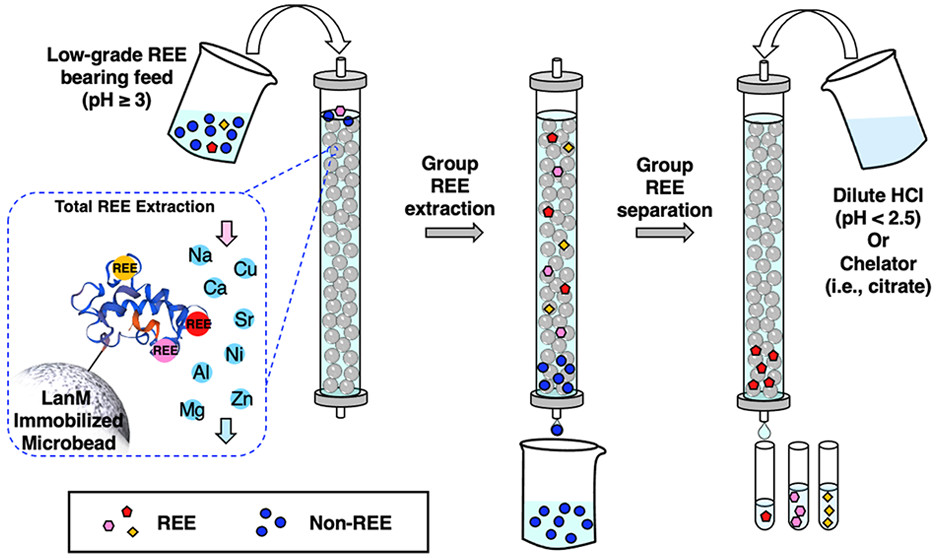
\includegraphics[width=0.9\textwidth]{./media/images/original_study_process}
    \caption{Overview of the work which inspired this thesis.
    Picture from "Bridging Hydrometallurgy and Biochemistry:
    A Protein-Based Process for Recovery and Separation of Rare Earth Elements", Dong et al.~\cite{originalstudy}.}
    \label{fig:original_study_process}
\end{figure}


This is a very clever process that even inspired this thesis.
However, this work is not easy to reproduce.
It requires costly chemicals and machinery, which only a company or a university can afford.
Therefore, it was not feasible at our school.
What must also be taken into consideration is that they used a genetically modified bacteria which produced the lanmodulin.
This step alone would take too long to achieve for a diploma thesis.

\vspace{2em}

Good et al. took another approach, which is surprisingly similar to our work.
Their basic idea was to let \emph{M. extorquens} grow in a solution which contains electronic waste (figure~\ref{fig:similar_work}) and find methods to increase the yield of this recycling method~\cite{similarwork}.
This approach is fairly similar to our own work.
However, this work did not inspire us because the paper was first published on December 27th 2023, when we already had worked three months on our project.

\begin{figure}[H]
    \centering
    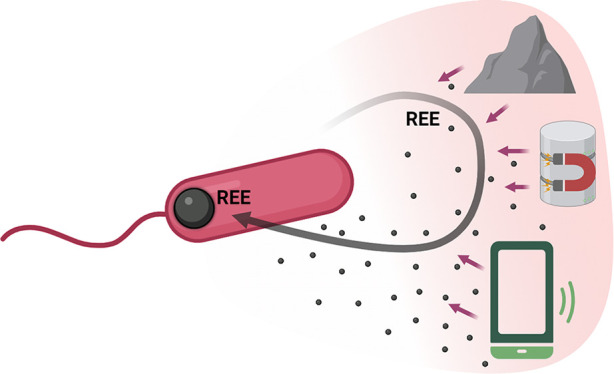
\includegraphics[width=0.9\textwidth]{./media/images/similar_work}
    \caption{Very simplified abstract of the work from Good et al.
    Picture from "Scalable and Consolidated Microbial Platform for Rare Earth Element Leaching and Recovery from Waste Sources", Good et al.~\cite{similarwork}.}
    \label{fig:similar_work}
\end{figure}

The main difference to our work is their technological advantage.
They used a genetically modified strain of \emph{M. extorquens} AM1, which is called \(\Delta\)\emph{mxaF}.
They deleted the gene \emph{mxaF} to ensure that the growth of the bacteria is dependent on the uptake of rare earths.
This led to a higher rare earth uptake capacity per bacteria.

Another remarkable difference is that they did not only let the bacteria grow with crushed magnets, but also with a crushed smartphone.
This did have, interestingly, no significant impact on the growth of \emph{M. extorquens} AM1 \(\Delta\)\emph{mxaF}, according to their study.

After that, they improved the yield by adding an organic acid to the bacteria's growth medium.
This helped to extract the rare earths from the crushed magnet (and smartphone).
What also boosted their yield was that they genetically engineered \emph{M. extorquens} AM1 \(\Delta\)\emph{mxaF} even further.

We can conclude that our project was done with the minimum of resources you can use to achieve some good results.
Compared to the above-mentioned studies, we had very limited resources and only basic laboratory equipment, so we could do only basic work.
What the other studies achieved is really great, but we showed that it is possible to be part of the newest developments of science without expensive materials and equipment.